
\documentclass[journal]{IEEEtran}

\usepackage{cite}
\usepackage{amsmath,amssymb,amsfonts}
\usepackage{algorithmic}
\usepackage{graphicx}
\usepackage{textcomp}
\usepackage{xcolor}

\usepackage{pgfplots} % per a graficar amb LaTeX
\pgfplotsset{samples=2000} % número màxim de punts d'una corba que genera ell, canviar
\pgfplotsset{compat=1.16} % perquè si no el pgfplot dóna error
\usepackage{import} % per a les imatges d'Inkscape
\usepackage{xifthen} % per a les imatges d'Inkscape
\usepackage{pdfpages} % per a les imatges d'Inkscape
\usepackage{transparent} % per a les imatges d'Inkscape
\usepackage[RPvoltages]{circuitikz} % per tal que no salti warning
\usetikzlibrary{arrows, decorations.markings, arrows.meta} % per a dibuixar fletxes d'intensitat
\usepackage{balance}
%\usepackage{flushend}
\usepackage{lettrine}



\begin{document}
%
% paper title
% Titles are generally capitalized except for words such as a, an, and, as,
% at, but, by, for, in, nor, of, on, or, the, to and up, which are usually
% not capitalized unless they are the first or last word of the title.
% Linebreaks \\ can be used within to get better formatting as desired.
% Do not put math or special symbols in the title.
\title{Alternating Search Directions Algorithm}
%
%
% author names and IEEE memberships
% note positions of commas and nonbreaking spaces ( ~ ) LaTeX will not break
% a structure at a ~ so this keeps an author's name from being broken across
% two lines.
% use \thanks{} to gain access to the first footnote area
% a separate \thanks must be used for each paragraph as LaTeX2e's \thanks
% was not built to handle multiple paragraphs
%

\author{Josep Fanals i Batllori,~\IEEEmembership{Student Member,~IEEE}
% \thanks{M. Shell was with the Department
% of Electrical and Computer Engineering, Georgia Institute of Technology, Atlanta,
% GA, 30332 USA e-mail: (see http://www.michaelshell.org/contact.html).}% <-this % stops a space
\thanks{J. Fanals i Batllori was with Universitat de Girona, 17003 Girona, Spain, (e-mail: jfanals13@gmail.com)}}

% note the % following the last \IEEEmembership and also \thanks - 
% these prevent an unwanted space from occurring between the last author name
% and the end of the author line. i.e., if you had this:
% 
% \author{....lastname \thanks{...} \thanks{...} }
%                     ^------------^------------^----Do not want these spaces!
%
% a space would be appended to the last name and could cause every name on that
% line to be shifted left slightly. This is one of those "LaTeX things". For
% instance, "\textbf{A} \textbf{B}" will typeset as "A B" not "AB". To get
% "AB" then you have to do: "\textbf{A}\textbf{B}"
% \thanks is no different in this regard, so shield the last } of each \thanks
% that ends a line with a % and do not let a space in before the next \thanks.
% Spaces after \IEEEmembership other than the last one are OK (and needed) as
% you are supposed to have spaces between the names. For what it is worth,
% this is a minor point as most people would not even notice if the said evil
% space somehow managed to creep in.



% The paper headers
\markboth{IEEE Transactions on Power Systems, Vol. XX, No. XX, XX 2020}{}%
% {Shell \MakeLowercase{\textit{et al.}}: Bare Demo of IEEEtran.cls for IEEE Journals}
% The only time the second header will appear is for the odd numbered pages
% after the title page when using the twoside option.
% 
% *** Note that you probably will NOT want to include the author's ***
% *** name in the headers of peer review papers.                   ***
% You can use \ifCLASSOPTIONpeerreview for conditional compilation here if
% you desire.




% If you want to put a publisher's ID mark on the page you can do it like
% this:
%\IEEEpubid{0000--0000/00\$00.00~\copyright~2015 IEEE}
% Remember, if you use this you must call \IEEEpubidadjcol in the second
% column for its text to clear the IEEEpubid mark.



% use for special paper notices
%\IEEEspecialpapernotice{(Invited Paper)}




% make the title area
\maketitle

% As a general rule, do not put math, special symbols or citations
% in the abstract or keywords.
\begin{abstract}
Typically, the power flow problem has been solved by means of iterative methods that either offer convenient convergence properties as well as robustness but lack simplicity or vice-versa. The Alternating Search Directions (ASD) approach has been presented as a novel algorithm suitable for power systems. It exploits their characteristics so that no Jacobian matrix is required. Thus, it becomes less complex while also it has been tested to be robust enough. Apart from detailing the method, this paper is aimed at discussing the convenience of the method not only for power systems but also for nonlinear equations involved in other kinds of electric applications. The paper also focuses on some techniques for adapting PV buses as there is not a unique approach. The results turn out to be heavily affected by this exact choice, as well as the selection of search directions. The IEEE14 and IEEE30 bus systems are employed as grid examples in order to show how the modeling of PV buses and modifications in the search directions can improve results. 
\end{abstract}

% Note that keywords are not normally used for peerreview papers.
\begin{IEEEkeywords}
alternating search directions, iterative solver, load flow, power system analysis computing, power system simulation.
\end{IEEEkeywords}

\IEEEpeerreviewmaketitle



\section{Introduction}
\IEEEPARstart{P}{ower} flow or load flow is likely the cornerstone problem in power systems. It gives a solution to all voltages, currents and powers in a given grid operating in a steady-state fashion. However, the equations that define the power flow are known to be nonlinear.

As a result of that, iterative methods have become the go-to tool to solve them. Some of the most basic ones are the Gauss-Seidel, which is appropriate for small size grids, and the popular Newton-Rapshon (NR) along with its variations, such as the Fast Decoupled Load Flow method \cite{hongfu},\cite{kothari},\cite{Stott}. The Newton-Raphson method converges quadratically. That causes it to converge to an acceptable solution with few iterations, hence its reputation \cite{gomez}.

Nevertheless, iterative solvers are not guaranteed to reach the operatively correct solution of the power system. By the nature of the power flow problem, there are several mathematically correct solutions. Depending on the selected seed, i.e. the initial value provided to the unknowns, iterative methods may converge to a non-feasible solution or in extreme cases they may even diverge \cite{11ill_tripathy},\cite{11ill_bonini}. Looking to ensure or increase the likelihood of finding the correct solution, a few methods have emerged in the last decades. Variations of the NR such as the usage of Iwamoto's multiplier and the Levenberg-Marquardt method, continuation power flow schemes, homotopy-based methods as well as the Holomorphic Embedding Load-Flow Method are some of them.

An initial variation of the NR method was based on the usage of Iwamoto's multiplier. At its core, it scales the Jacobian matrix by a factor called the optimal step size parameter, which has to be found. Despite requiring more iterations than the classic NR, it has been proven to work better for ill-conditioned systems \cite{iwamoto}. Another variation consists in the Levenberg-Marquardt method. It can be thought of as an algorithm that instead of employing the Jacobian as such, it adjusts it by trying to minimize the sum of active and reactive powers squared \cite{lagace},\cite{milano}. Like the Iwamoto deviation, it needs more iterations than the classical NR. Moreover, none of these deviations escapes from computing and factorizing the Jacobian matrix. 

The continuation power flow scheme is concerned about finding the power-voltage curves around the saddle-nose bifurcation point (SNBP), also called the voltage collapse point. This point establishes the limit between the stable and the unstable operation of the system, and between the high-voltage and the low-voltage solution as well. Despite its correct performance, the algorithm may be computationally demanding as it departs from a flat start or more generally, an operating situation far from the final one \cite{11ill_bonini}. Thus, it iterates in several points to draw the full curve while still being tied to the Jacobian.

Homotopy-based methods are commonly used to find the multiple DC operating points of an electronic circuit consisting of thousands of transistors \cite{yamamura},\cite{trajkovic}. They consist in adding the $\lambda$ parameter and adapting the equations depending on the chosen kind of homotopy. When $\lambda=0$ the system of equations is easily solved and it constitutes a starting point. Then, $\lambda$ is treated as an unknown, and whenever $\lambda=1$ a new solution is found. Power systems can also benefit from a method based on homotopy, as seen in \cite{mehta}. Mainly, all solutions mathematically possible in a given grid can be found. On the downside, it still requires a Jacobian matrix and of course, more time to compute the results.

The Holomorphic Embedding Load-Flow Method (HELM) has been regarded as a robust novel method that constructs the solution recursively \cite{Trias2012}. It has been stated that when the power flow solution exists, HELM finds it unequivocally, whereas when it does not, the method is able to signal it thanks to Sigma approximants. This capacity to diagnose the state of the grid makes it unique, since NR-like algorithms certainly cannot \cite{Trias2018}, \cite{Trias_sigma}. In addition to that, Thévenin approximants are a resource meant to compute both power flow solutions around the SNBP, although the negative branch result may suffer from poor precision \cite{Trias2018}. The inclusion of PV buses considered in \cite{Schmidt}, \cite{Subramanian} caused numerical problems, yet their modeling has been improved in \cite{Trias2018}, \cite{Rao}, \cite{subramanianPV}. Overall HELM is a convenient method with the negative aspect of encountering convolutions and a rather complex formulation \cite{Trias2018}.

The Alternating Search Directions method (ASD) was introduced in \cite{asd} as a generalization of the Gauss-Seidel and NR methods. Its main distinction is found in not depending on the Jacobian matrix and being able to adapt the search directions to converge to the high-voltage solution. It takes advantage of the nature of power systems to divide the problem into two parts. Each part of the problem evolves to the next by following a predefined direction, different from the other one. These directions can be understood as constant matrices. Thus, in terms of speed it is much faster than NR \cite{asd}, and more than everything else, simpler.

This paper is mainly concerned with the treatment of PV nodes to accelerate the convergence, as the choice in \cite{asd} is not unique. The paper also points at a mistake found in \cite{asd}, proposes changes in the search directions and explains the suitability of the method for a wider range of applications. 

The outline of this work is as follows: Section \ref{sec1} introduces the ASD method; Section \ref{sec2} covers the modifications to take into account in order to improve the convergence of the algorithm; Section \ref{sec3} explains ASD's particular attributes and discusses whether or not it is suitable for other applications; finally, Section \ref{sec4} concludes the paper.


\section{The ASD algorithm} \label{sec1}
Surprisingly, the Alternating Search Directions method as such is not new. In essence, it was employed decades ago to solve heat transfer problems \cite{Rimek}, structural mechanics \cite{ladeveze} and grid equations \cite{samarskii}. It was only recently applied to power systems in \cite{asd}, where more details about the method that will be explained here will be found. 

ASD is described by a two-step process. First, an intermediate solution is obtained by solving the linear system:
\begin{equation}
  \begin{cases}
    I^{l+\frac{1}{2}} - I^l = \alpha(V^{l+\frac{1}{2}} - V^l),\\
    YV^{l + \frac{1}{2}} = I_0 + I^{l+\frac{1}{2}},
  \end{cases}
  \label{eq:step1}
\end{equation}
where $I$ stands for currents, $V$ for voltages, $Y$ is the bus admittance matrix, $I_0$ represents the slack bus current contribution and $\alpha$ a matrix that defines the first search direction. The index $l$ indicates a given iteration and the intermediate solution is denoted by $l+\frac{1}{2}$. Selecting a suitable $\alpha$ matrix is key, as it will remain the same during the calculation process. This step relies on the linearity of $Y$. 

Once the intermediate solution is found, the second step obeys:
\begin{equation}
  \begin{cases}
    I^{l+1} - I^{l+\frac{1}{2}} = \beta(V^{l+1} - V^{l+\frac{1}{2}}),\\
    (V^{l+1})^*I^{l+1}=S^*,
  \end{cases}
  \label{eq:step2}
\end{equation}
where $S^*$ is the conjugated power injection at each bus and $\beta$ a matrix responsible for establishing the second search direction. It shares dimensions with $\alpha$ and is equally important. Like in the first step, in the second step the system of equations imposed by \eqref{eq:step2} has to be solved in closed form. This step is also called the local step, where instead of using the information provided by the bus admittance matrix, is takes into consideration the complex power in each bus.

It is assumed that the active and reactive power of each and every bus that constitutes the system (apart from the slack bus) is known. In other words, all buses are PQ except for the slack bus, so PV buses have not been treated as of now. As it has already been stated, \eqref{eq:step2} can be solved in a non-iterative manner. However, the last equation provided in \cite{asd} contains an incorrect sign. If $A=[(Y-\beta)V^{l+\frac{1}{2}}-I_0]/\beta$, $U=V^{l+1}/A$ and $\Sigma=-S^*/(AA^*\beta)$, the high-voltage solution is given by:
\begin{equation}
  U=\frac{-1-\sqrt{1-4(\Im(\Sigma)^2+\Re(\Sigma))}}{2}+j\Im({\Sigma}).
  \label{eq:Uerrors}
\end{equation}
In contrast with the authors' statements, the negative root has to be chosen because of how $\Sigma$ was defined. 

The inclusion of PV buses is achieved by working with the PV sensitivity matrix, where the reactive power injected in a given PV bus depends on variations of current and voltage at the intermediate step. Previously, $Y$ is divided through a Kron reduction, where $Y_{11}$ denotes the links only between PQ buses, $Y_{22}$ between PV buses and $Y_{12}$ and $Y_{21}$ the connections between the two different types of buses. First the voltage variations are computed considering its current phase and the difference between the datum absolute value $E_{PV}$:
\begin{equation}
  \Delta V^{l+\frac{1}{2}} = (E_{PV}-|V^{l+\frac{1}{2}}|)V^{l+\frac{1}{2}}/|V^{l+\frac{1}{2}}|.
  \label{eq:incrV}
\end{equation}
Then, knowing $\Delta V^{l+\frac{1}{2}}$, current variations are computed as seen from PV buses:
\begin{equation}
  \Delta I^{l+\frac{1}{2}}=(Y_{22}+Y_{21}Y^{-1}_{11}Y_{12})\Delta V^{l + \frac{1}{2}}.
  \label{eq:incrI}
\end{equation}
Finally, the new reactive power for PV buses at the global step follows:
\begin{equation}
  Q^{l+1}=Q^l+\gamma \Im(V^l(\Delta I^{l+\frac{1}{2}})^*),
  \label{eq:Qdef}
\end{equation}
where $\gamma$ is an added parameter needed to relax the variations so that the discriminant in \eqref{eq:Uerrors} turns out to be positive in each iteration. It is not uncommon to be forced to employ $\gamma<0.1$. As it can be derived, it plays a crucial role when looking for adequate convergence properties. An excessive $\gamma$ results in not obtaining a valid solution from \eqref{eq:Uerrors} whereas if $\gamma$ becomes too small, the algorithm converges much slower than desired.

\subsection{Results}
The IEEE14 and the IEEE30-bus system have been selected in order to test how the original ASD method performs. Although the IEEE14 grid contains several off-nominal tap ratio transformers, there is no special modeling to consider. Both grids are formed by PQ as well as PV buses.

For the IEEE14 system, the most convenient value for $\gamma$ has been found by a trial and error approach to be around 0.24. The evolution of the maximum power mismatch as a function of iterations and $\gamma$ is shown in Fig. \ref{fig:0}. In the logarithmic y-axis, the maximum error decays linearly. The number of iterations is superior to what the typical NR would need since it converges quadratically. As a rule of thumb, it usually needs no more than 5 iterations \cite{kothari}.


\begin{figure}[!ht]\footnotesize
\centering
\begin{tikzpicture}
    \begin{axis}[
        /pgf/number format/.cd, ylabel={$\log|\Delta S_{max}|$},xlabel={Number of iterations},domain=-0.25:0.25,legend style={at={(0,0)},anchor=south west},width=9cm,height=6.5cm,scatter/classes={%
        a={mark=x, mark size=0.001pt, draw=green}, b={mark=x,mark size=1.0pt,draw=black}, c={mark=x,mark size=1.0pt,draw=black}, d={mark=o,mark size=1.0pt,draw=black}}]]
        \addplot[densely dashed]%
        table[x = x, y = y, meta = label, col sep=semicolon] {Data/err_14_02.csv};
        \addplot[ densely dashdotted]%
        table[x = x, y = y, meta = label, col sep=semicolon] {Data/err_14_022.csv};
        \addplot[densely dotted]%
        table[x = x, y = y, meta = label, col sep=semicolon] {Data/err_14_024.csv};
        \addplot[ solid]%
        table[x = x, y = y, meta = label, col sep=semicolon] {Data/err_14_026.csv};

        \legend{$\gamma=0.20$, $\gamma=0.22$, $\gamma=0.24$,$\gamma=0.26$}
    \end{axis}
    \end{tikzpicture}
\caption{Maximum errors depending on the number of iterations and $\gamma$ for the IEEE14-bus grid.}
\label{fig:0}
\end{figure}

On the other hand, adjusting $\gamma$ properly is not only convenient but mandatory. For instance, for the IEEE14-bus system when $\gamma>0.35$ the algorithm does not progress because of the negative discriminant in \eqref{eq:Uerrors}. The IEEE30-bus grid is arguably more well-conditioned than the IEEE14-bus system. This can be studied thanks to the Sigma plot given by HELM's Sigma approximants. Because of that, for $\gamma>0.10$ the algorithm starts suffering from the aforementioned problems. In this case the ideal $\gamma$ is close to 0.07.

Thus, $\gamma$ has to be understood as an under-relaxation parameter \cite{asd} that becomes smaller the more well-conditioned the system is. It implies that the reactive power injection in PV buses is reduced because the absolute values $E_{PV}$ can be mantained. In ill-conditioned systems $\gamma$ will tend to increase. Table \ref{tab:0} shows the dependence between the loading factor $\lambda$, which scales all known powers, and $\gamma$. The results sustain the previous discussion. Still, the variation of $\gamma$ is modest.

\begin{table}[!ht]
  % increase table row spacing, adjust to taste
  \renewcommand{\arraystretch}{1.3}
  \caption{Optimal under-relaxation parameter depending on the loading factor}
  \label{tab:0}
  \centering
  \begin{tabular}{ccc}
  \hline
  % & \multicolumn{2}{c}{Embedding}\\
  % \cline{2-3}
  $\lambda$ & IEEE14 & IEEE30\\
  \hline
  0.25 & 0.19 & 0.06\\
  0.75 & 0.22 & 0.06\\
  1.00 & 0.24 & 0.07\\
  1.50 & 0.24 & 0.08\\
  2.00 & 0.30 & 0.08\\
  \hline
  \end{tabular}
  \end{table} 

The trajectory that the evolution of $Q^{l+1}$ describes is highly related to $\gamma$. There are three main paths it can follow. The ideal one is when $\gamma$ turns out to be limited enough so that the reactive power stabilizes and converges to the solution. The second possible outcome is more problematic, in the sense that the reactive power remains unstable, changing its sign often. The remaining case has to do with finding a negative discriminant in \eqref{eq:Uerrors}. In this case, the algorithm becomes unable to make progress. Fig. \ref{fig:1} exemplifies this pattern of behavior for bus number 26 of the IEEE30-bus system while $\lambda=1.00$.

\begin{figure}[!ht]\footnotesize
  \centering
  \begin{tikzpicture}
      \begin{axis}[
          /pgf/number format/.cd, ylabel={$Q^{l+1}_{26}$},xlabel={Number of iterations},domain=-0.25:0.25,legend style={at={(1,0)},anchor=south east},width=9cm,height=6.5cm,scatter/classes={%
          a={mark=x, mark size=0.001pt, draw=green}, b={mark=x,mark size=1.0pt,draw=black}, c={mark=x,mark size=1.0pt,draw=black}, d={mark=o,mark size=1.0pt,draw=black}}]]
          \addplot[densely dashed]%
          table[x = x, y = y, meta = label, col sep=semicolon] {Data/Q_30_007.csv};
          \addplot[densely dashdotted]%
          table[x = x, y = y, meta = label, col sep=semicolon] {Data/Q_30_010.csv};
          \addplot[densely dotted]%
          table[x = x, y = y, meta = label, col sep=semicolon] {Data/Q_30_011.csv};
          \legend{$\gamma=0.07$, $\gamma=0.10$, $\gamma=0.11$}
      \end{axis}
      \end{tikzpicture}
  \caption{The three sets of possible $Q^{l+1}_{26}$ trajectories for several values of $\gamma$.}
  \label{fig:1}
  \end{figure}

As it can be derived from Fig. \ref{fig:1}, the path of the reactive power is highly sensitive to changes in $\gamma$. For instance, in the extreme case of $\gamma=0.11$ at the iteration number 15 the algorithm encounters a negative root. That is why $\gamma$ has to be carefully adjusted by hand. Intuition about the system is widely welcomed; in the beginning, there are no obvious values to use. Employing an exagerated value like $\gamma=0.11$ results in noticing the problem, whereas $\gamma=0.10$ does not signal the issue. 

It has to be noted that the results obtained in this subsection have been generated by considering $\alpha=diag(S^*/|V_b|^2)$, where it has been assumed that the base voltage $|V_b|=1$, and $\beta=diag(Y-\alpha)$. This choice is critical and it will be reviewed in Section \ref{sec2}.

\section{Modifications to improve convergence} \label{sec2}
Neither the treatment of PV buses nor the selection of $\alpha$ and $\beta$ is unique. The authors in \cite{asd} tested the algorithm for several choices of $\alpha$ and $\beta$ but the PV bus modeling remained always the same. In this paper a new way of treating control buses is introduced. It will be compared to the one in \cite{asd}. Then, the search directions defined by $\alpha$ and $\beta$ will be modified.

% ara introduir el mètode Santiago (el que tinc al fitxer v7santiago), veure com respon i a quant ajustar gamma. Després canviar les matrius alpha i beta

\subsection{PV bus modeling}
The PV sensitivity matrix is capable of yielding satisfactory results as can be observed in Fig. \ref{fig:0}. However, it needs to go through a three-step process where first of all the algorithm computes voltage variations \eqref{eq:incrV}, then the current ones \eqref{eq:incrI} and finally updates the reactive power \eqref{eq:Qdef}. Initially a Kron reduction of the full bus admittance matrix $Y$ is required.

A much straightforward approach consists in scaling the voltages according to its actual absolute value and $E_{PV}$ and then consider that its phase remains constant:
\begin{equation}
  V^{l+\frac{1}{2}} := V^{l+\frac{1}{2}} \frac{E_{PV}}{|V^{l+\frac{1}{2}}|}.
  \label{eq:Vnou}
\end{equation}
Essentially it is the same as \eqref{eq:incrV} with the only difference that in this case there is no interest in computing the variation but rather the value as such. The next step uses the linearity imposed by the transmission lines and transformers, which all together build the $Y$ matrix. Expanding the calculation of the complex power $S=VI*$ results in:
\begin{equation}
  Q^{l+\frac{1}{2}}=\Im(V^{l+\frac{1}{2}}(Y_{PV}V^{l+\frac{1}{2}} - I_0)^*),
  \label{eq:Qnou}
\end{equation}
where the matrix $Y_{PV}=[Y_{21}, Y_{22}]$.
Updating the reactive power this way could cause trouble as its variations could be extreme. Hence, it is also convenient to use the under-relaxation parameter:
\begin{equation}
  Q^{l+1}=Q^{l} + \gamma_2 (Q^{l+\frac{1}{2}} - Q^l).
  \label{eq:Qnou2}
\end{equation}
This way, once $Q^{l+\frac{1}{2}} - Q^l\rightarrow 0$, $Q^{l+1} - Q^l\rightarrow 0$ so reactive powers will tend to converge, just like they would with \eqref{eq:Qdef}.

To test this new choice of modeling PV buses, the IEEE14 and the IEEE30-bus systems have been selected. The under-relaxation parameter (called $\gamma_2$ for the new treatment instead of $\gamma$) has also been adjusted to the optimal value. As it can be appreciated from Fig. \ref{fig:2}, its response becomes superior to the original modeling in \cite{asd}, especially for the IEEE14-bus system.  

\begin{figure}[!ht]\footnotesize
  \centering
  \begin{tikzpicture}
      \begin{axis}[
          /pgf/number format/.cd, ylabel={$\log|\Delta S_{max}|$},xlabel={Number of iterations},domain=-0.25:0.25,legend style={at={(1,1)},anchor=north east},width=9cm,height=6.5cm,scatter/classes={%
          a={mark=x, mark size=0.001pt, draw=green}, b={mark=x,mark size=1.0pt,draw=black}, c={mark=x,mark size=1.0pt,draw=black}, d={mark=o,mark size=1.0pt,draw=black}}]]
          \addplot[densely dashed]%
          table[x = x, y = y, meta = label, col sep=semicolon] {Data/err_2_14_024.csv};
          \addplot[densely dashdotted]%
          table[x = x, y = y, meta = label, col sep=semicolon] {Data/errS_2_14_040.csv};
          \addplot[densely dotted]%
          table[x = x, y = y, meta = label, col sep=semicolon] {Data/err_2_30_007.csv};
          \addplot[solid]%
          table[x = x, y = y, meta = label, col sep=semicolon] {Data/errS_2_30_012.csv};
  
          \legend{$\gamma=0.24$ (14), $\gamma_2=0.40$ (14), $\gamma=0.07$ (30), $\gamma_2=0.12$ (30)}
      \end{axis}
      \end{tikzpicture}
  \caption{Maximum errors depending on the number of iterations for the IEEE14 - represented by (14) - and the IEEE30-bus - symbolized by (30) -  grids with both PV modeling options.}
  \label{fig:2}
  \end{figure}

As found in \cite{asd}, the ASD method can be an order of magnitude faster than the classic NR. By applying this new modeling of PV buses even fewer iterations are required in order to obtain similar mismatches. The calculation of the new reactive power is not substantially more computationally intense than the original choice. Therefore, needing fewer iterations translates directly to a slightly faster algorithm in comparison to the one in \cite{asd}, so in this aspect, it is also way superior to the NR.

\subsection{Adjustment of search directions}
The search directions constitute two key matrices: $\alpha$ and $\beta$. Both are customizable and there is no a priori better choice. It has been shown that depending on their values, the ASD ends up resembling methods as the Gauss-Seidel, NR or the Implicit Z bus algorithm \cite{asd}. In other words, the alternating search directions can be considered a generalization of some well-known numerical methods.

Anyway, one of the main advantages ASD has above the other numerical methods has to do with avoiding the Jacobian matrix, and because of that, it makes sense to aim at constructing convenient $\alpha$ and $\beta$ matrices. The authors in \cite{asd} build $\alpha$ as a diagonal matrix formed by the conjugated complex power of each bus. It could be divided for the squared base voltage, although $V_b$ tends to approximate 1, so qualitatively speaking it does not make much of a difference. On the other hand, $\beta$ is also a diagonal matrix generated in this case from computing the bus admittance matrix minus $\alpha$. Remarkable enough, $\alpha$ takes into account the complex power while at the same time it is considered in the global step where voltages and currents are related by the bus admittance matrix; $\beta$ is taken into account in the local step, even though it becomes responsible for relating voltages and currents partially by diagonal bus admittance elements. In short, the definition of $\alpha$ compensates for the lack of 'locality' whereas $\beta$ does it for the lack of 'globality'.

In order to improve the convergence rate, adding a factor has been proven to accelerate it. The main aspect is that by increasing $\alpha$ and $\beta$ the under-relaxation parameter $\gamma_2$ can increase. Therefore, the unknown reactive power stabilizes faster. The proposed definition of the search directions turns out to be:
\begin{equation}
  \begin{cases}
    \alpha &= \psi diag(S^* / |V_b|^2),\\
    \beta &= \psi diag(Y+\alpha),
  \end{cases}
  \label{eq:alpha_beta}
\end{equation}
where the added parameter $\psi$ is the aforementioned factor and the only difference compared to \cite{asd}, except for the changing the sign of $\alpha$ in the $\beta$ definition.

Combining the new modeling of PV buses along with \eqref{eq:alpha_beta} leads to the improvements captured by Table \ref{tab:1}. It looks at the maximum mismatch at the arbitrary iteration number 30 for both grids and compares the results obtained with $\psi=1$ (the same as the ones in Fig. \ref{fig:2}) and the most appropriate $\psi$ and $\gamma_2$ values.

\begin{table}[!ht]
  % increase table row spacing, adjust to taste
  \renewcommand{\arraystretch}{1.3}
  \caption{Maximum error depending on $\psi$ and $\gamma_2$ in the 30th iteration}
  \label{tab:1}
  \centering
  \begin{tabular}{ccc|ccc}
  \hline 
  \multicolumn{3}{c}{IEEE14} & \multicolumn{3}{|c}{IEEE30}\\
    % \cline{1-3}  \cline{4-6} 
  $\psi$ & $\gamma_2$ & $\log|\Delta S_{max}|$ & $\psi$ & $\gamma_2$ & $\log|\Delta S_{max}|$\\
  % \hline
  \cline{1-3}  \cline{4-6}
  1.00 & 0.40 & 2.94e-08 & 1.00 & 0.12 & 2.48e-04\\
  2.01 & 0.55 & 4.68e-11 & 10.00 & 0.34 & 3.49e-07\\
  \hline
  \end{tabular}
  \end{table} 

From Table \ref{tab:1} it is clear that increasing $\psi$ and adjusting $\gamma_2$ properly results in an algorithm substantially faster than the one where matrices $\alpha$ and $\beta$ are given by the proposed methodology in \cite{asd}. Even more, it has been shown before that the new PV bus treatment provides a clear advantage in comparison to the usage of the PV bus sensitivity matrix. All in all, employing $\psi$ and modeling PV buses as described in this paper results in a superior ASD method than the one \cite{asd}. The main drawback is that $\psi$ has to be tuned depending on the system.

\section{Range of applications}\label{sec3}
As stated, the alternating search directions concept has been employed before for scientific domains that exclude power systems \cite{Rimek}, \cite{samarskii}, \cite{ladeveze}. Power systems have the particular characteristic that the connections between buses other than the ground or reference bus, whose voltage is set at 0 in every case, is linear. That is, the parameters of transformers and transmission lines are fully known. On the contrary, the connection between a given bus and the ground bus is nonlinear due to having $S=VI^*$. Nonetheless, this nonlinearity allows to solve the local step in closed form with \eqref{eq:Uerrors}. So, fortunately, the nature of power systems allows the ASD method to be a fitting choice. 

Nevertheless, in modern power systems not always the data linking buses is known beforehand. Power systems can benefit from the addition of FACTS, AC/DC converters and overall, components that have to do with power electronics \cite{arrillaga}. For instance, AC/DC converters constitute a well-know situation in which the converters add several unknowns to the nonlinear system of equations \cite{alvarez1}, \cite{alvarez2}, \cite{alvarez3}. As a consequence, the system has to expand to incorporate the corresponding equations, where the bus admittance matrix is not constant per se, as it depends on the converter unknowns. The ASD method would not be convenient for these kind of problems.

Another limitation of the ASD method is found in trying to accommodate it to solve integrated circuits potentially consisting of hundreds if not thousands of transistors and diodes. Integrated circuits simulators (SPICE-like programs) adapt the equations following the so-called modified nodal analysis approach \cite{hajj}. Their solutions are based on the NR method. It is virtually impossible to extend the usage of the ASD for such circuits since the connections between buses (or nodes) is defined by nonlinear elements. 

All this implies that the ASD method in its current form becomes confined to power systems where the unions between buses are completely known. A positive aspect of the ASD method is that different loads could be employed, such as exponential ones, as long as their current only depends on their voltage \cite{asd}. 


\section{Conclusion}\label{sec4}
This paper has introduced a new methodology to model PV buses convenient for the alternating search directions. It has been shown to be a satisfactory contribution, as the under-relaxation parameter $\gamma$ can be increased, accelerating the algorithm's convergence. Moreover, the matrices $\alpha$ and $\beta$ can also take advantage of slight modifications. These two aspects lead to power mismatches several orders of magnitude smaller compared to the original formulation when using the same number of iterations for the IEEE14 and the IEEE30-bus systems. At the same time, the algorithm keeps being similarly computationally intensive. 

The range of applicability of the alternating search directions is limited to solving the power flow of traditional power systems where no electronic components are added. Because of that, the strength of the method is found in solving the power flow problem fast and precisely enough. All this makes it a potential competitor to the DC load flow method, widely employed for contingency analysis. The alternating search directions method would provide a fast non-approximate result.



% use section* for acknowledgment
\section*{Acknowledgment}
The author would like to thank Santiago Peñate Vera for introducing and discussing the method in great depth. This paper would not have been written without him.


% \ifCLASSOPTIONcaptionsoff
%   \newpage
% \fi

\begin{thebibliography}{31}

\bibitem{hongfu}
W. Hongfu, M. Shixia, W. Yi and Z Zhihqiang, "An Approximate Power Flow Method to Deal with the Non-convergence Problem of Power Flow Calculation," in \emph{2018 International Conference on Power System Technology (POWERCON)}, Guangzhou, 2018, pp. 292-299.

\bibitem{kothari}
D. P. Kothari and I. J. Nagrath, "Modern Power System Analysis," 4th ed. New Dehli, Tata McGraw-Hill, 2011.

\bibitem{Stott}  
B. Stott, "Review of load-flow calculation methods," in \emph{Proceedings of the IEEE}, vol. 62, no. 7, pp. 916-929, July 1974. 

% \bibitem{Novel}
% H. Chiang, T. Wang and H. Sheng, "A novel fast and flexible holomorphic embedding power flow method," in \emph{IEEE Transactions on Power Systems}, vol. 33, no. 3, pp. 2551-2562, May 2018.

\bibitem{gomez}
A. Gomez-Exposito and C. Gomez-Quiles, "Factorized load flow," in \emph{IEEE Transactions on Power Systems}, vol. 28, no. 4, pp. 4607-4614. Nov. 2013.

\bibitem{11ill_tripathy}
S. C. Tripathy, G. D. Prasad, O. P. Malik and G. S. Hope, "Load-flow solutions for ill-conditioned power systems by a Newton-like method," in \emph{IEEE Transactions on Power Apparatus and Systems}, vol. PAS-101, no. 10, pp. 3648-3657, Oct. 1982.

\bibitem{11ill_bonini}
A. Bonini Neto, R. R. Matarucco, and D. A. Alves, "Technique for continuation power flow using the “flat start” and for ill-conditioned systems," in \emph{World Journal Control Science and Engineering}, no. 1, pp. 1-7, 2015.

\bibitem{iwamoto}
S. Iwamoto, Y. Tamura, "A load flow calculation method for ill-conditioned power systems," in \emph{IEEE transactions on power apparatus and systems}, vol. PAS-100, no. 4. pp. 1736-1743, 1981.

\bibitem{lagace}
P. J. Lagace, M. H. Vuong and I. Kamwa, "Improving power flow convergence by Newton Raphson with a Levenberg-Marquardt method," \emph{2008 IEEE Power and Energy Society General Meeting - Conversion and Delivery of Electrical Energy in the 21st Century}, Pittsburgh, PA, 2008, pp. 1-6.

\bibitem{milano}
F. Milano, "Analogy and Convergence of Levenberg's and Lyapunov-Based Methods for Power Flow Analysis," in \emph{IEEE Transactions on Power Systems}, vol. 31, no. 2, pp. 1663-1664, 2016.

\bibitem{yamamura}
K. Yamamura, T. Sekiguchi and Y. Inoue, "A fixed-point homotopy method for solving modified nodal equations," in \emph{IEEE Transactions on Circuits and Systems I: Fundamental Theory and Applications}, vol. 46, no. 6, pp. 654-665, 1999.

\bibitem{trajkovic}
L. Trajkovic, E. Fung and S. Sanders, "HomSPICE: simulator with homotopy algorithms for finding DC and steady-state solutions of nonlinear circuits," \emph{1998 IEEE International Symposium on Circuits and Systems (ISCAS)}, Monterey, CA, 1998, pp. 227-231 vol.6.

\bibitem{mehta}
D. Mehta, H. Nguyen and K. Turitsyn, "Numerical Polynomial Homotopy Continuation Method to Locate All The Power Flow Solutions," arXiv:1408.2732v1, Aug. 2014.

\bibitem{Trias2012}
A. Trias, "HELM: the Holomorphic Embedding Load-Flow Method," \emph{2012 IEEE Power and Energy Society General Meeting}, San Diego, CA, 2012, pp. 1-8.

\bibitem{Trias2018}
A. Trias, "HELM: The Holomorphic Embedding Load-Flow Method. Foundations and Implementations," \emph{Foundations and Trends\textsuperscript{\textregistered} in Electric Energy Systems}, vol. 3, no. 3-4, pp. 140-370, 2018.

\bibitem{Trias_sigma}
A. Trias, "Sigma algebraic approximants as a diagnostic tool in power networks," \emph{U.S. Patent}. 9563722 B2, Feb. 7, 2017.

\bibitem{Schmidt}
B. Schmidt, "Implementation and evaluation of the holomorphic embedding load flow method," M.S. Thesis, Dept. Elec. Eng., Tech. Univ. of Munich, Munich, Germany, 2015.

\bibitem{Subramanian}
M. K. Subramanian, "Application of holomorphic embedding to the power-flow problem," M.S. Thesis, Arizona State Univ., Tempe, AZ, USA, 2014.

% \newpage
% \IEEEtriggercmd{\enlargethispage{1in}}
% \IEEEtriggeratref{9}

\bibitem{Rao}
S. Rao, "Exploration of a scalable holomorphic embedding method formulation for power system analysis applications," Ph.D. dissertation, Arizona State Univ., Tempe, AZ, USA, 2017.

\bibitem{subramanianPV}
M. K. Subramanian, Y. Feng and D. Tylavsky, "PV bus modeling in a holomorphically embedded power-flow formulation," \emph{2013 North American Power Symposium (NAPS)}, Manhattan, KS, 2013, pp. 1-6.

\bibitem{asd}
D. Borzacchiello, F. Chinesta, H. Malik, R. García-Blanco and P. Díez, "Unified formulation of a family of iterative solvers for power systems analysis," in \emph{Electric Power Systems Research}, vol. 140, pp. 201–208, 2016.

\bibitem{Rimek}
F. F. Rimek, "Method of alternating directions for the solution of parabolic equations with a convective term," in \emph{Journal of engineering physics}, vol. 21, pp. 1450-1456, 1971.

\bibitem{samarskii}
A. A. Samarskii and E. S. Nikolaev, "Numerical Methods for Grid Equations", Volume II Iterative Methods, Birkhäuser Basel, 1989.

\bibitem{ladeveze}
P. Ladeveze and J. Simmonds, "Nonlinear Computational Structural Mechanics: New Approaches and Non-Incremental Methods of Calculation", Mechanical Engineering Series, New York, Springer, 1999.

\bibitem{arrillaga}
J. Arrillaga and B. Smith, "AC-DC Power System Analysis", The Institution of Electrical Engineers, London, UK, 1998.

\bibitem{alvarez1}
(To Be Published) A. Alvarez-Bustos, B. Kazemtabrizi, M. Shahbazi and R. D. Zimmerman, "MATPOWER-FUBM: Flexible Universal Branch Model for Matpower’s Optimal Power Flow and Power Flow Tools for Hybrid AC/DC Power Systems Research and Education," in \emph{Power Systems, IEEE Transactions on}, vol. XX, no. X, pp. XX–XX, Month. 20XX.  

\bibitem{alvarez2}
(Under Review) A. Alvarez-Bustos, B. Kazemtabrizi, M. Shahbazi and E. Acha-Daza, "Universal Branch Model for the Solution of Optimal Power Flows in Hybrid AC/DC Grids," in \emph{International Journal of Electrical Power and Energy Systems}, vol. XX, no. X, pp. XX–XX, Month. 20XX. 

\bibitem{alvarez3}
A. Alvarez-Bustos (2020). MATPOWER-FUBM (Version 1.0) [Software]. Available at https://github.com/AbrahamAlvarezB/matpower-fubm.

\bibitem{zimmerman}
R. D. Zimmerman, C. E. Murillo-Sanchez and R. J. Thomas, "MATPOWER: Steady-State Operations, Planning and Analysis Tools for Power Systems Research and Education," in \emph{IEEE Transactions on Power Systems}, vol. 26, no. 1, pp. 12-19, Feb. 2011.

\bibitem{zimmerman2}
R. D. Zimmerman and C. E. Murillo-Sanchez (2019). MATPOWER (Version 7.0) [Software]. Available at https://matpower.org.

\bibitem{hajj}
I. N. Hajj, "Extended Nodal Analysis," in \emph{IEEE Transactions on Computer-Aided Design of Integrated Circuits and Systems}, vol. 31, no. 1, pp. 89-100, 2012.

\newpage
\IEEEtriggercmd{\enlargethispage{1in}}
\IEEEtriggeratref{30}

\bibitem{meseguer}
A. Meseguer, "Fundamentals of Numerical Mathematics for physicists and engineers", Hoboken, NJ, Wiley, 2020.



\end{thebibliography}

\begin{IEEEbiography}[{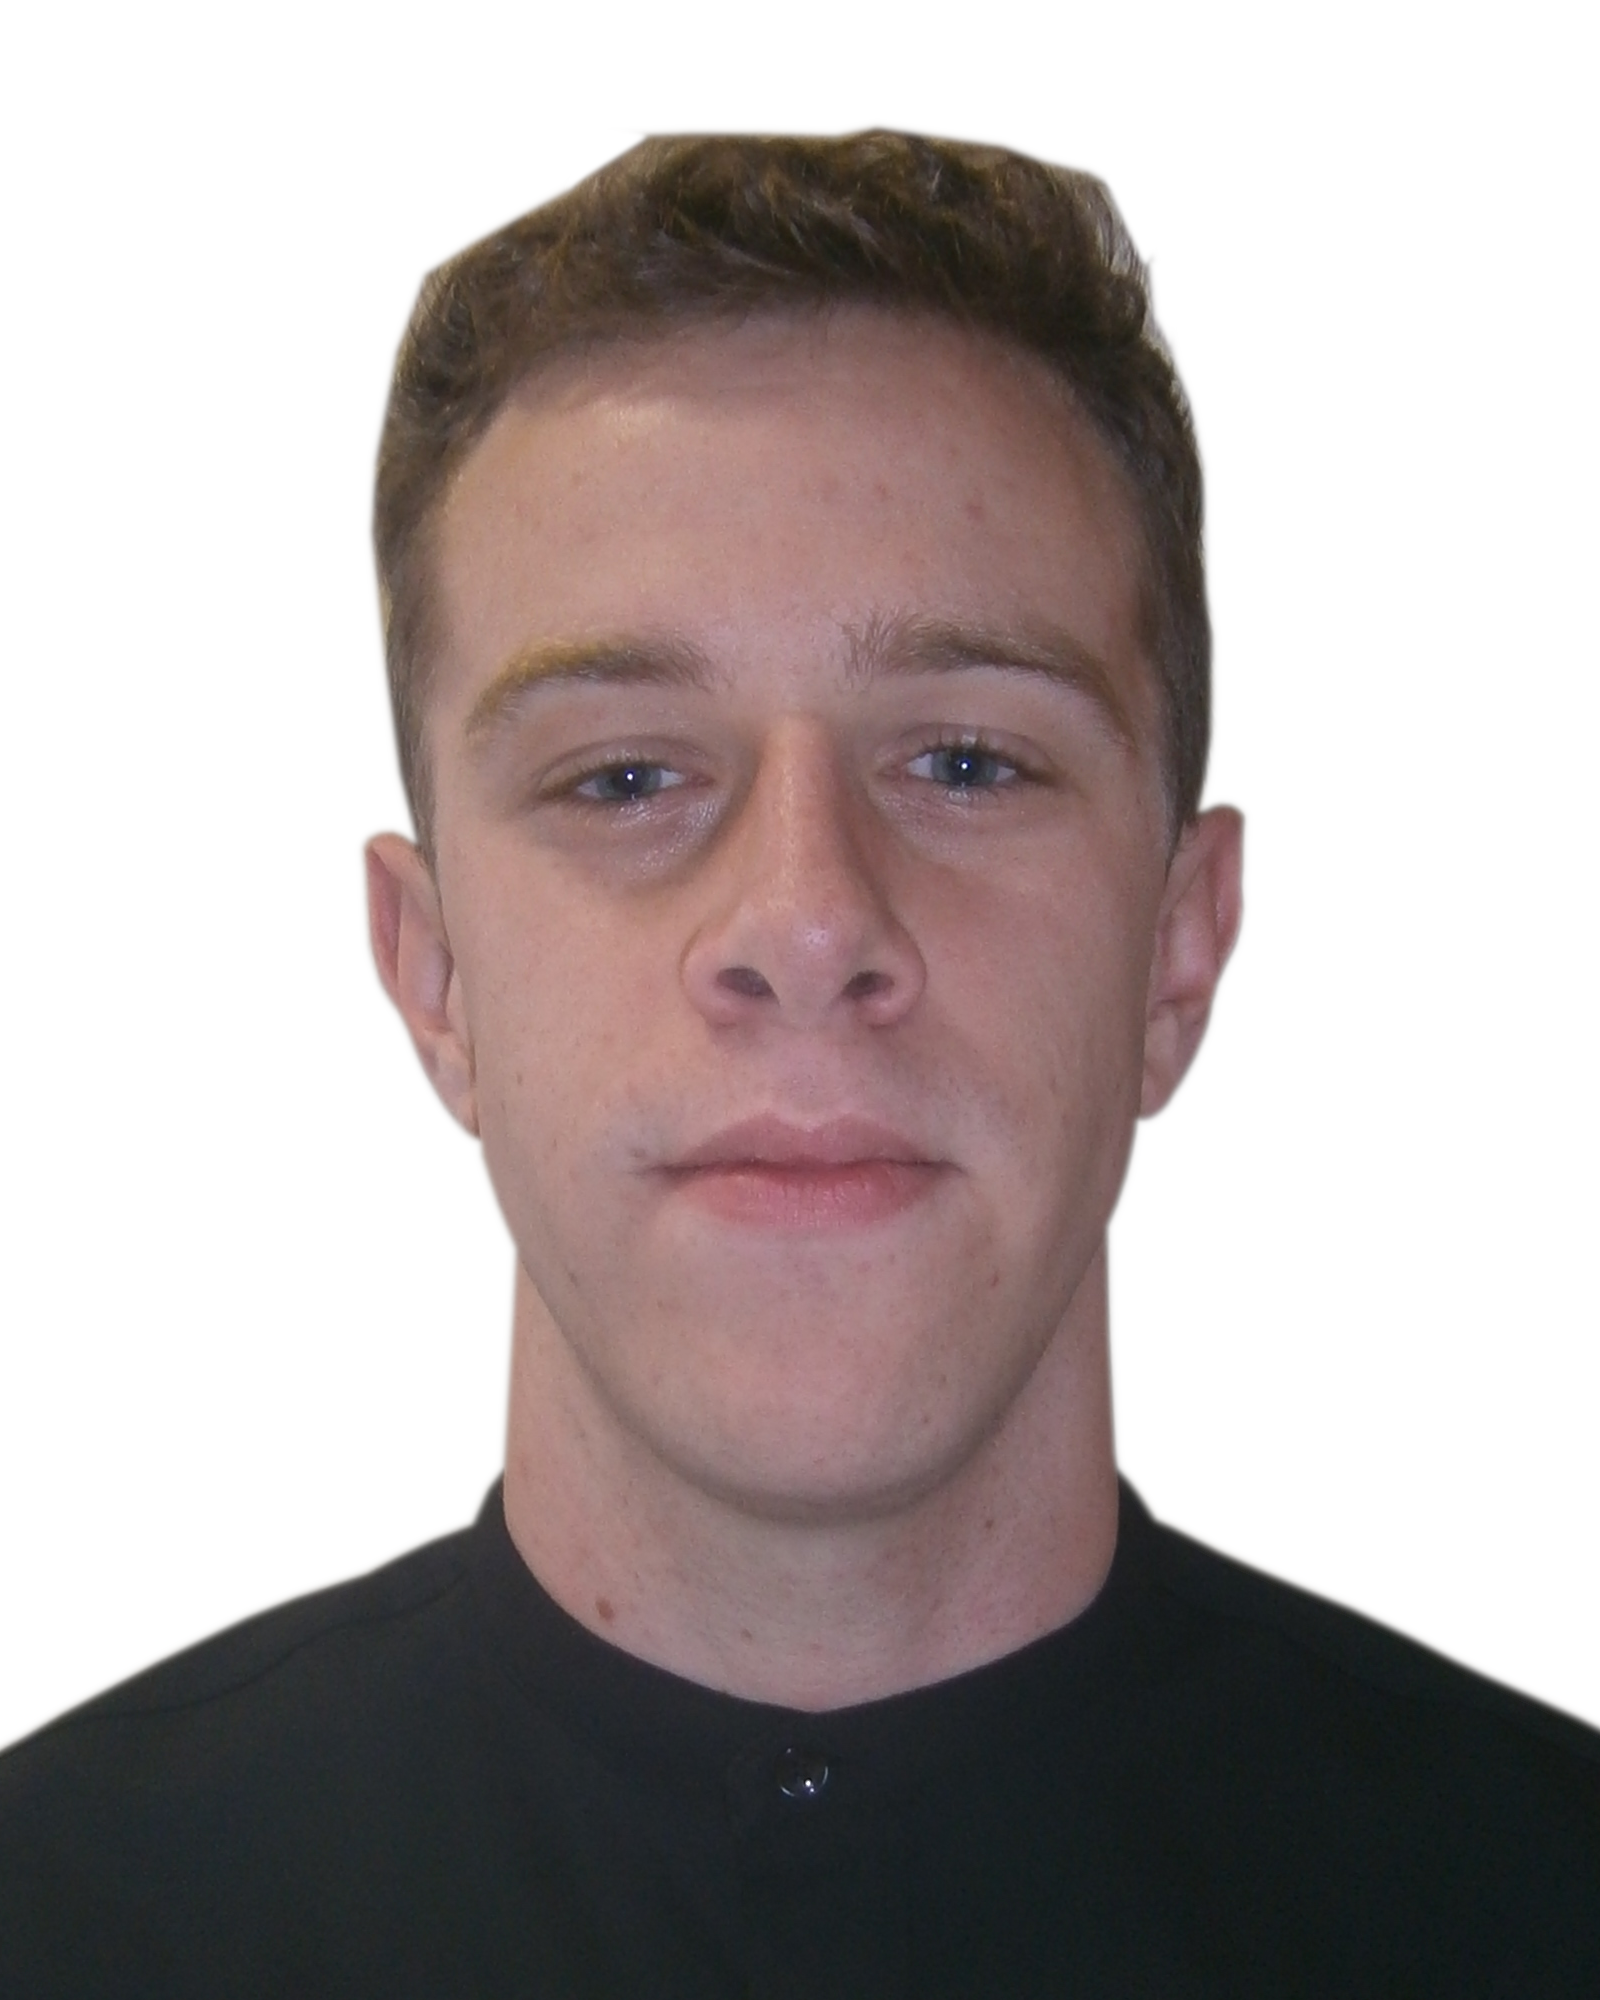
\includegraphics[width=1in,height=1.25in,clip,keepaspectratio]{Data/Imatge.png}}]{Josep Fanals i Batllori}
was born in la Bisbal d'Empordà, Spain, in 1998. He received the B.S. degree in electrical engineering from the Universitat de Girona, Girona, Spain, in 2020. His primary area of interest is the study of techniques to solve the power flow problem.
\end{IEEEbiography}



\vfill

% insert where needed to balance the two columns on the last page with
% biographies
%\newpage

% \begin{IEEEbiographynophoto}{Jane Doe}
% Biography text here.
% \end{IEEEbiographynophoto}

% You can push biographies down or up by placing
% a \vfill before or after them. The appropriate
% use of \vfill depends on what kind of text is
% on the last page and whether or not the columns
% are being equalized.

%\vfill

% Can be used to pull up biographies so that the bottom of the last one
% is flush with the other column.
%\enlargethispage{-5in}



% that's all folks
\end{document}


